NetFlow and \ac{IPFIX} are the two popular protocols for IP flow information
export. NetFlow \cite{rfc3954} is a network protocol designed by Cisco
Systems, which allows routers to generate and export flow records to a
designated collector. \ac{IPFIX} \cite{rfc5101} on the other hand is an open
standard by IETF based on NetFlow v$9$. The novelty of the standard lies in
its ability to describe record formats at runtime using templates based on an
extensible and well-defined information model. The data transfer mechanism is
also simplistic and extensible by being unidirectional and transport protocol
agnostic.

The wide applicability of this approach is easily seen from the pervasive use
of flow records for a vibrant set of network analysis applications. For
instance, a survey by Sperotto \textit{et al.} \cite{sperotto:2010} gives an
overview of how network flow analysis can be used to detect Denial of Service
attacks, scan probing target systems and the target discovery phase of worms.
In addition, a survey by Callado \textit{et al.} \cite{callado:2009} also
lists behaviour analysis of Internet backbone traffic and general anomaly
detection.

Understanding intricate traffic patterns require sophisticated flow analysis
tools that can mine flow records for such a usage.  Unfortunately current
tools fail to deliver owing to their language design and simplistic filtering
methods.  We recently proposed a flow query language design
\cite{vmarinov:2009} that aims to cater to such needs.  It can process
flow records, aggregate them into groups, apply absolute or relative filters
and invoke Allen interval algebra rules \cite{fallen:1983}. The expressiveness
of the language can be seen from \cite{vperelman:2011} where the authors
formulate flow queries to identify flow signatures of popular applications.

Flowy \cite{kkanev:2010} was a first feature complete Python prototype of that
flow query language. Due to performance problems, it was superseeded by a
complete rewrite in C, called Flowy 2.0 \cite{jschauer:thesis:2011}. In this
paper, we introduce \ac{NFQL} which extends on Flowy 2.0, making it more
feature complete and optimizing its execution engine with crispier algorithms.
We show that this iteration of our work is able to scale to real-world sized
traces and has comparable execution times to contemporary flow analysis tools.

The paper is organized as follows. In section \ref{sec:relatedwork} we survey
the current state-of-the-art flow-processing tools and reason how \ac{NFQL} is
different from each one of them. In section \ref{sec:design} we describe the
flow query language by discussing each stage of the processing pipeline. In
section \ref{sec:implementation} we introduce the inner workings of \ac{NFQL}.
It begins by providing an overview of the \ac{NFQL} architecture and the
structure of the intermediate format used to exchange messages. The workflow of
the execution engine is described next and is supplemented by a number of
performance optimizations made to make the implementation scale. The section is
followed by performance evaluations comparing \ac{NFQL} against contemporary
flow processing tools alongwith with a discussion on its current limitation and
future outlook in section \ref{sec:evaluation}, with conclusion in section
\ref{sec:conclusion}.

\begin{figure*}[!t]
\centering
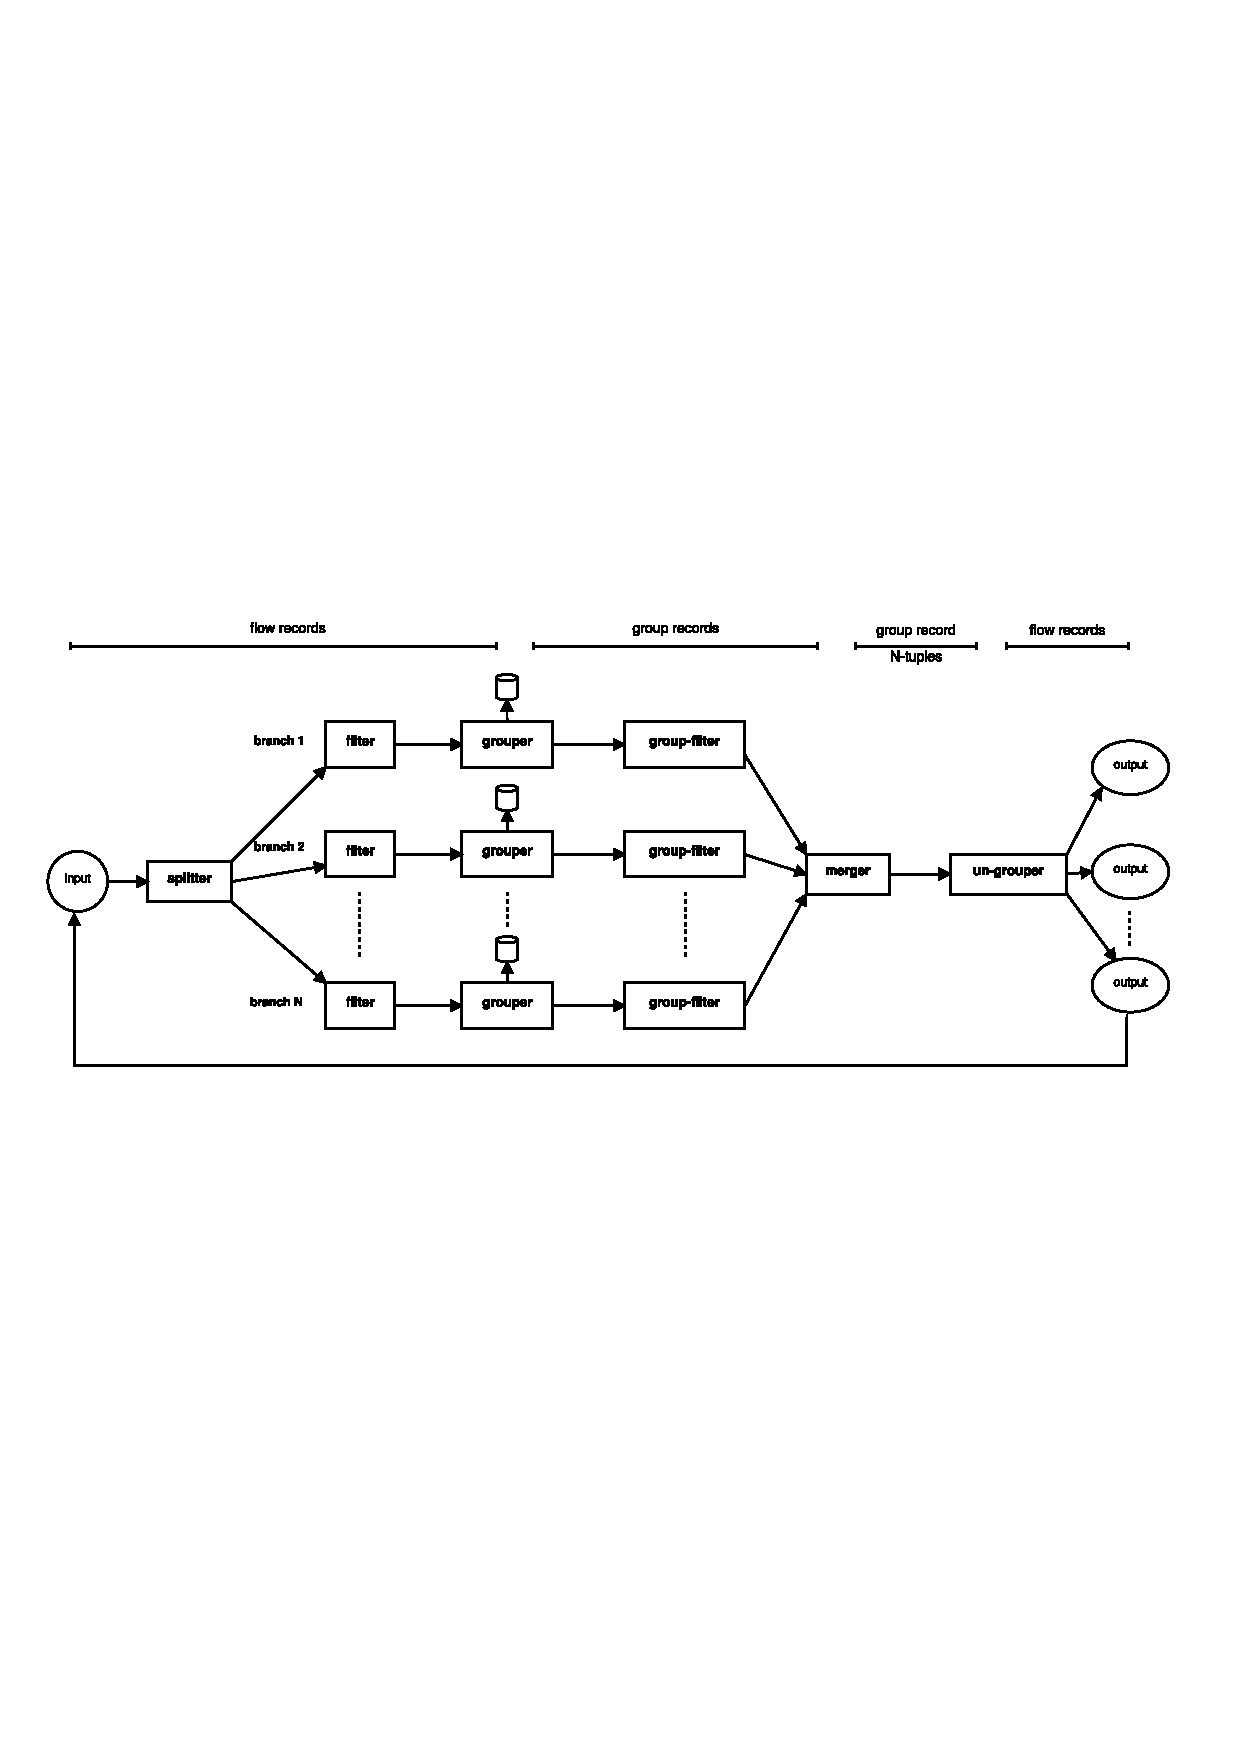
\includegraphics[width=0.9\linewidth]{nfql-pipeline}
\caption{NFQL Processing Pipeline \cite{vmarinov:2009}}
\label{fig:nfql-pipeline}
\end{figure*}
